% !TEX root = /Users/ramunnoj/fiji/BlobTracker User Manual/manual.tex

\section{2D time series}
\begin{figure}[h]
\centering
	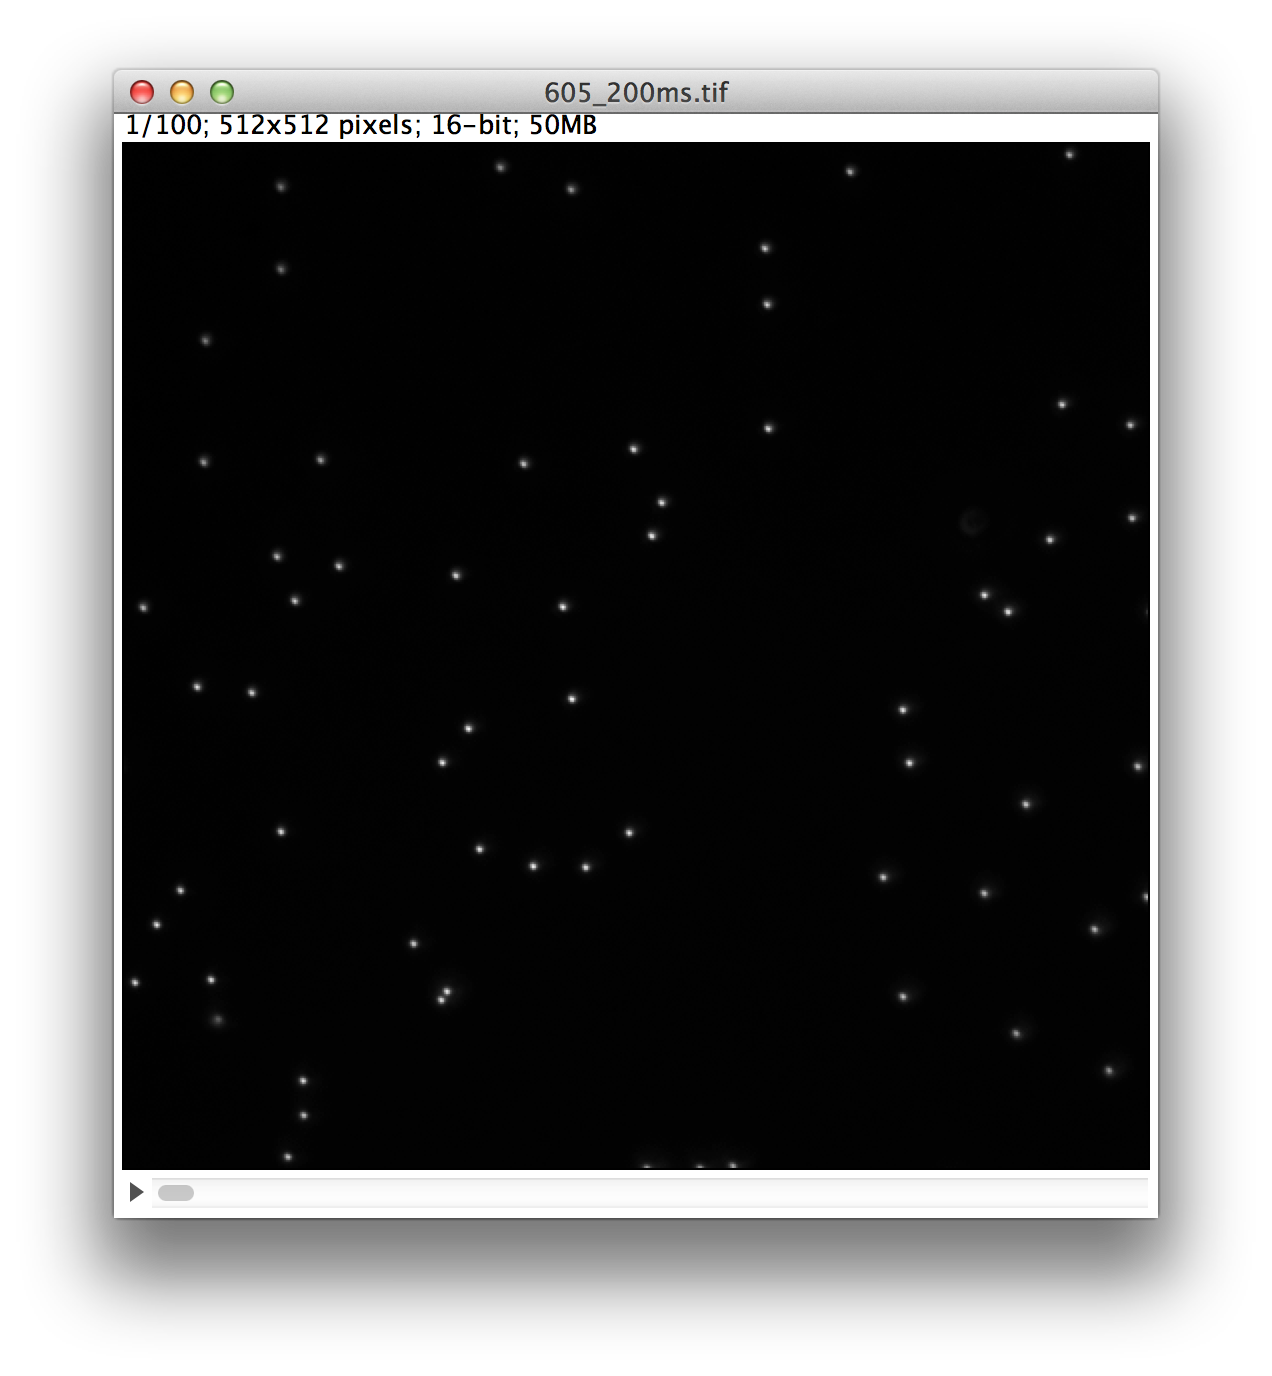
\includegraphics[width=4 in]{stack.png}
	\caption{Load image stack}
	\label{stack}
\end{figure}

\begin{figure}[h]
\centering
	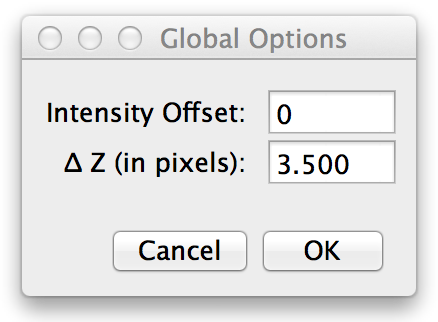
\includegraphics[width=3 in]{openWindow1.png}
	\caption{Enter intensity offset, and $\Delta$Z ratio. Ratio only maters for 3D data}
	\label{window1}
\end{figure}

\begin{figure}[h]
\centering
	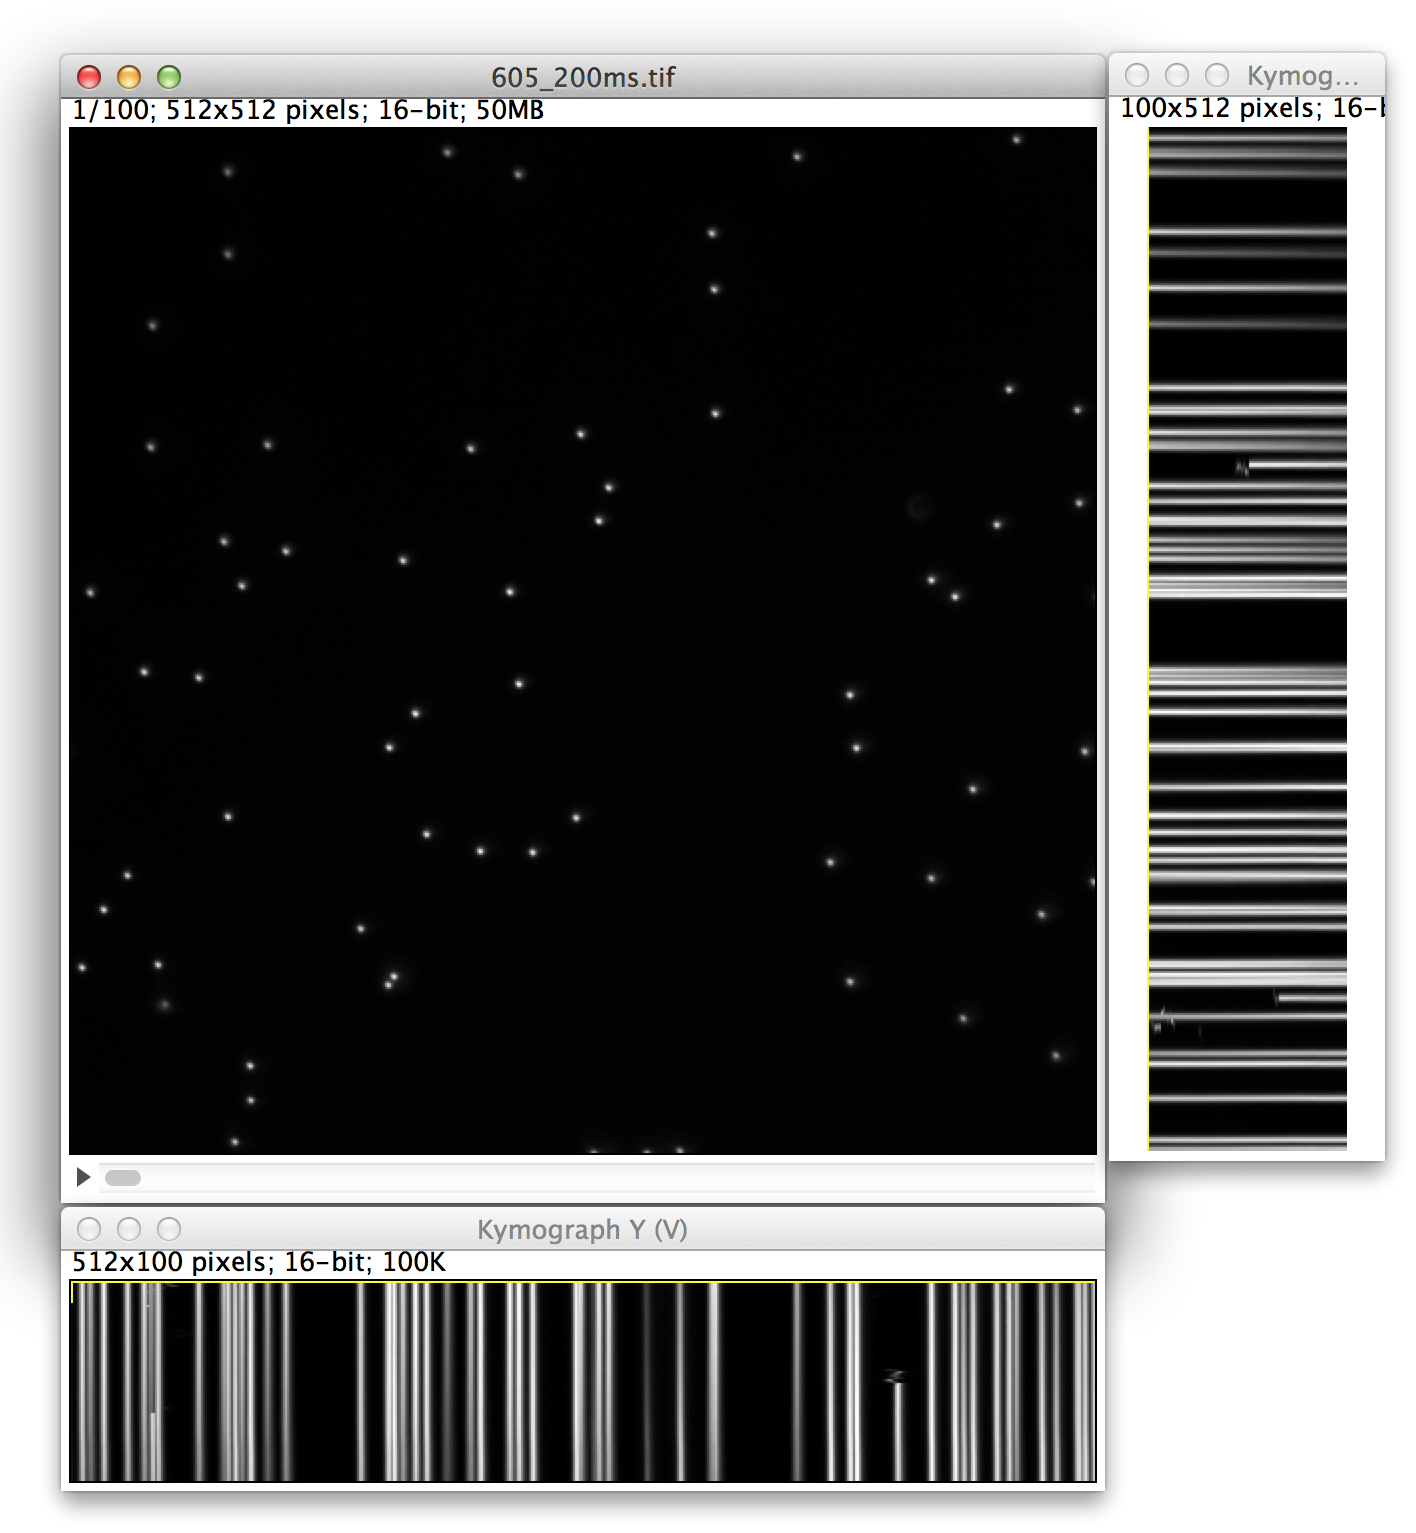
\includegraphics[width=4 in]{image2D.png}
	\caption{The 2D image stack now has x and y kymographs}
	\label{image2D}
\end{figure}

\begin{figure}[h]
\centering
	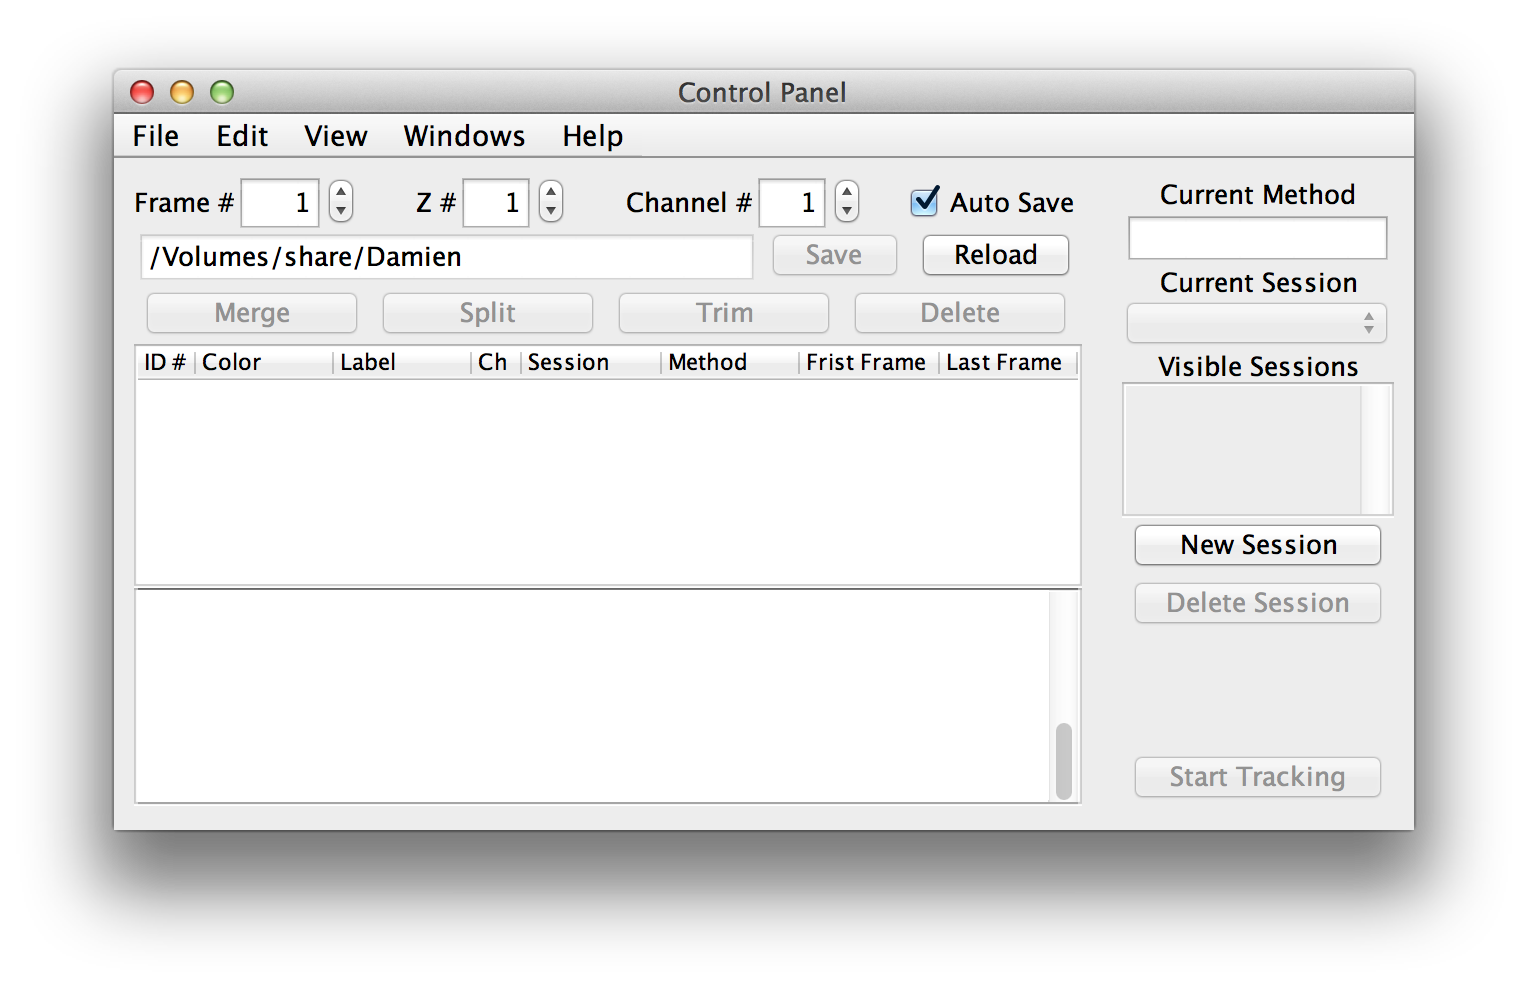
\includegraphics[width=4 in]{controlWindow.png}
	\caption{This is the control window}
	\label{controlWindow}
\end{figure}

\begin{figure}[h]
\centering
	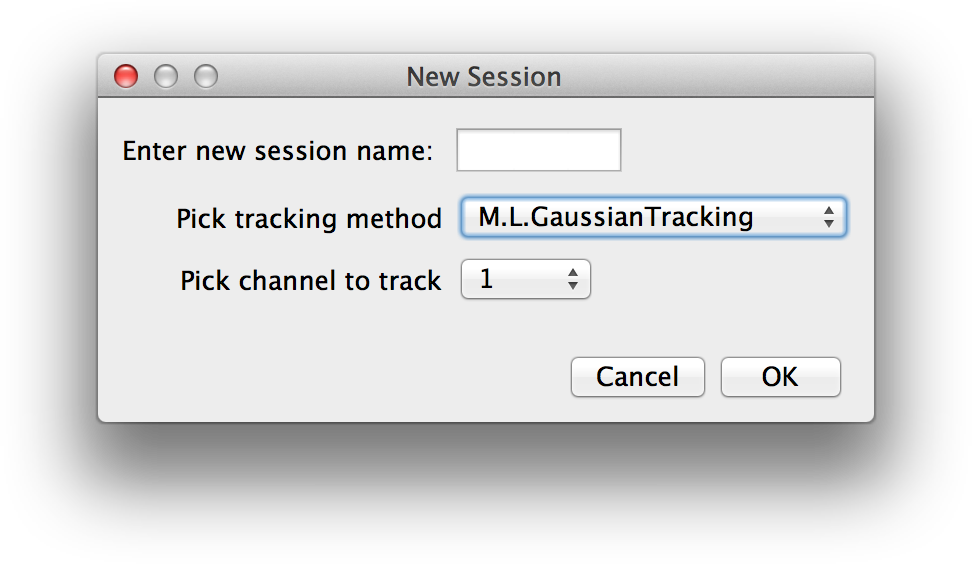
\includegraphics[width=4 in]{newSession.png}
	\caption{Enter session name, then pick tracking method, and then pick data channel to apply tracking method to.}
	\label{newSession}
\end{figure}


\begin{figure}[h]
\centering
	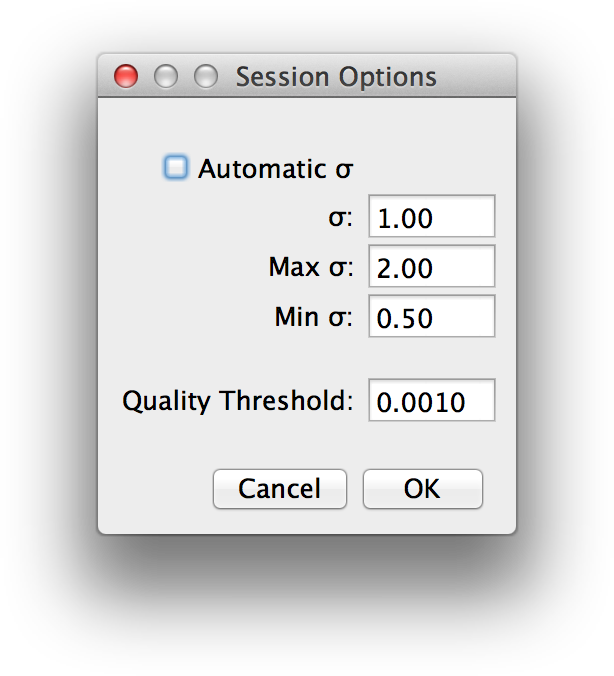
\includegraphics[width=3 in]{sessionOptions.png}
	\caption{Pick options for tracking method. Software can pick $\sigma$ automatically, or you can enter the values.  You can also adjust the threshold for tracking. }
	\label{sessionOptions}
\end{figure}

\begin{figure}[h]
\centering
	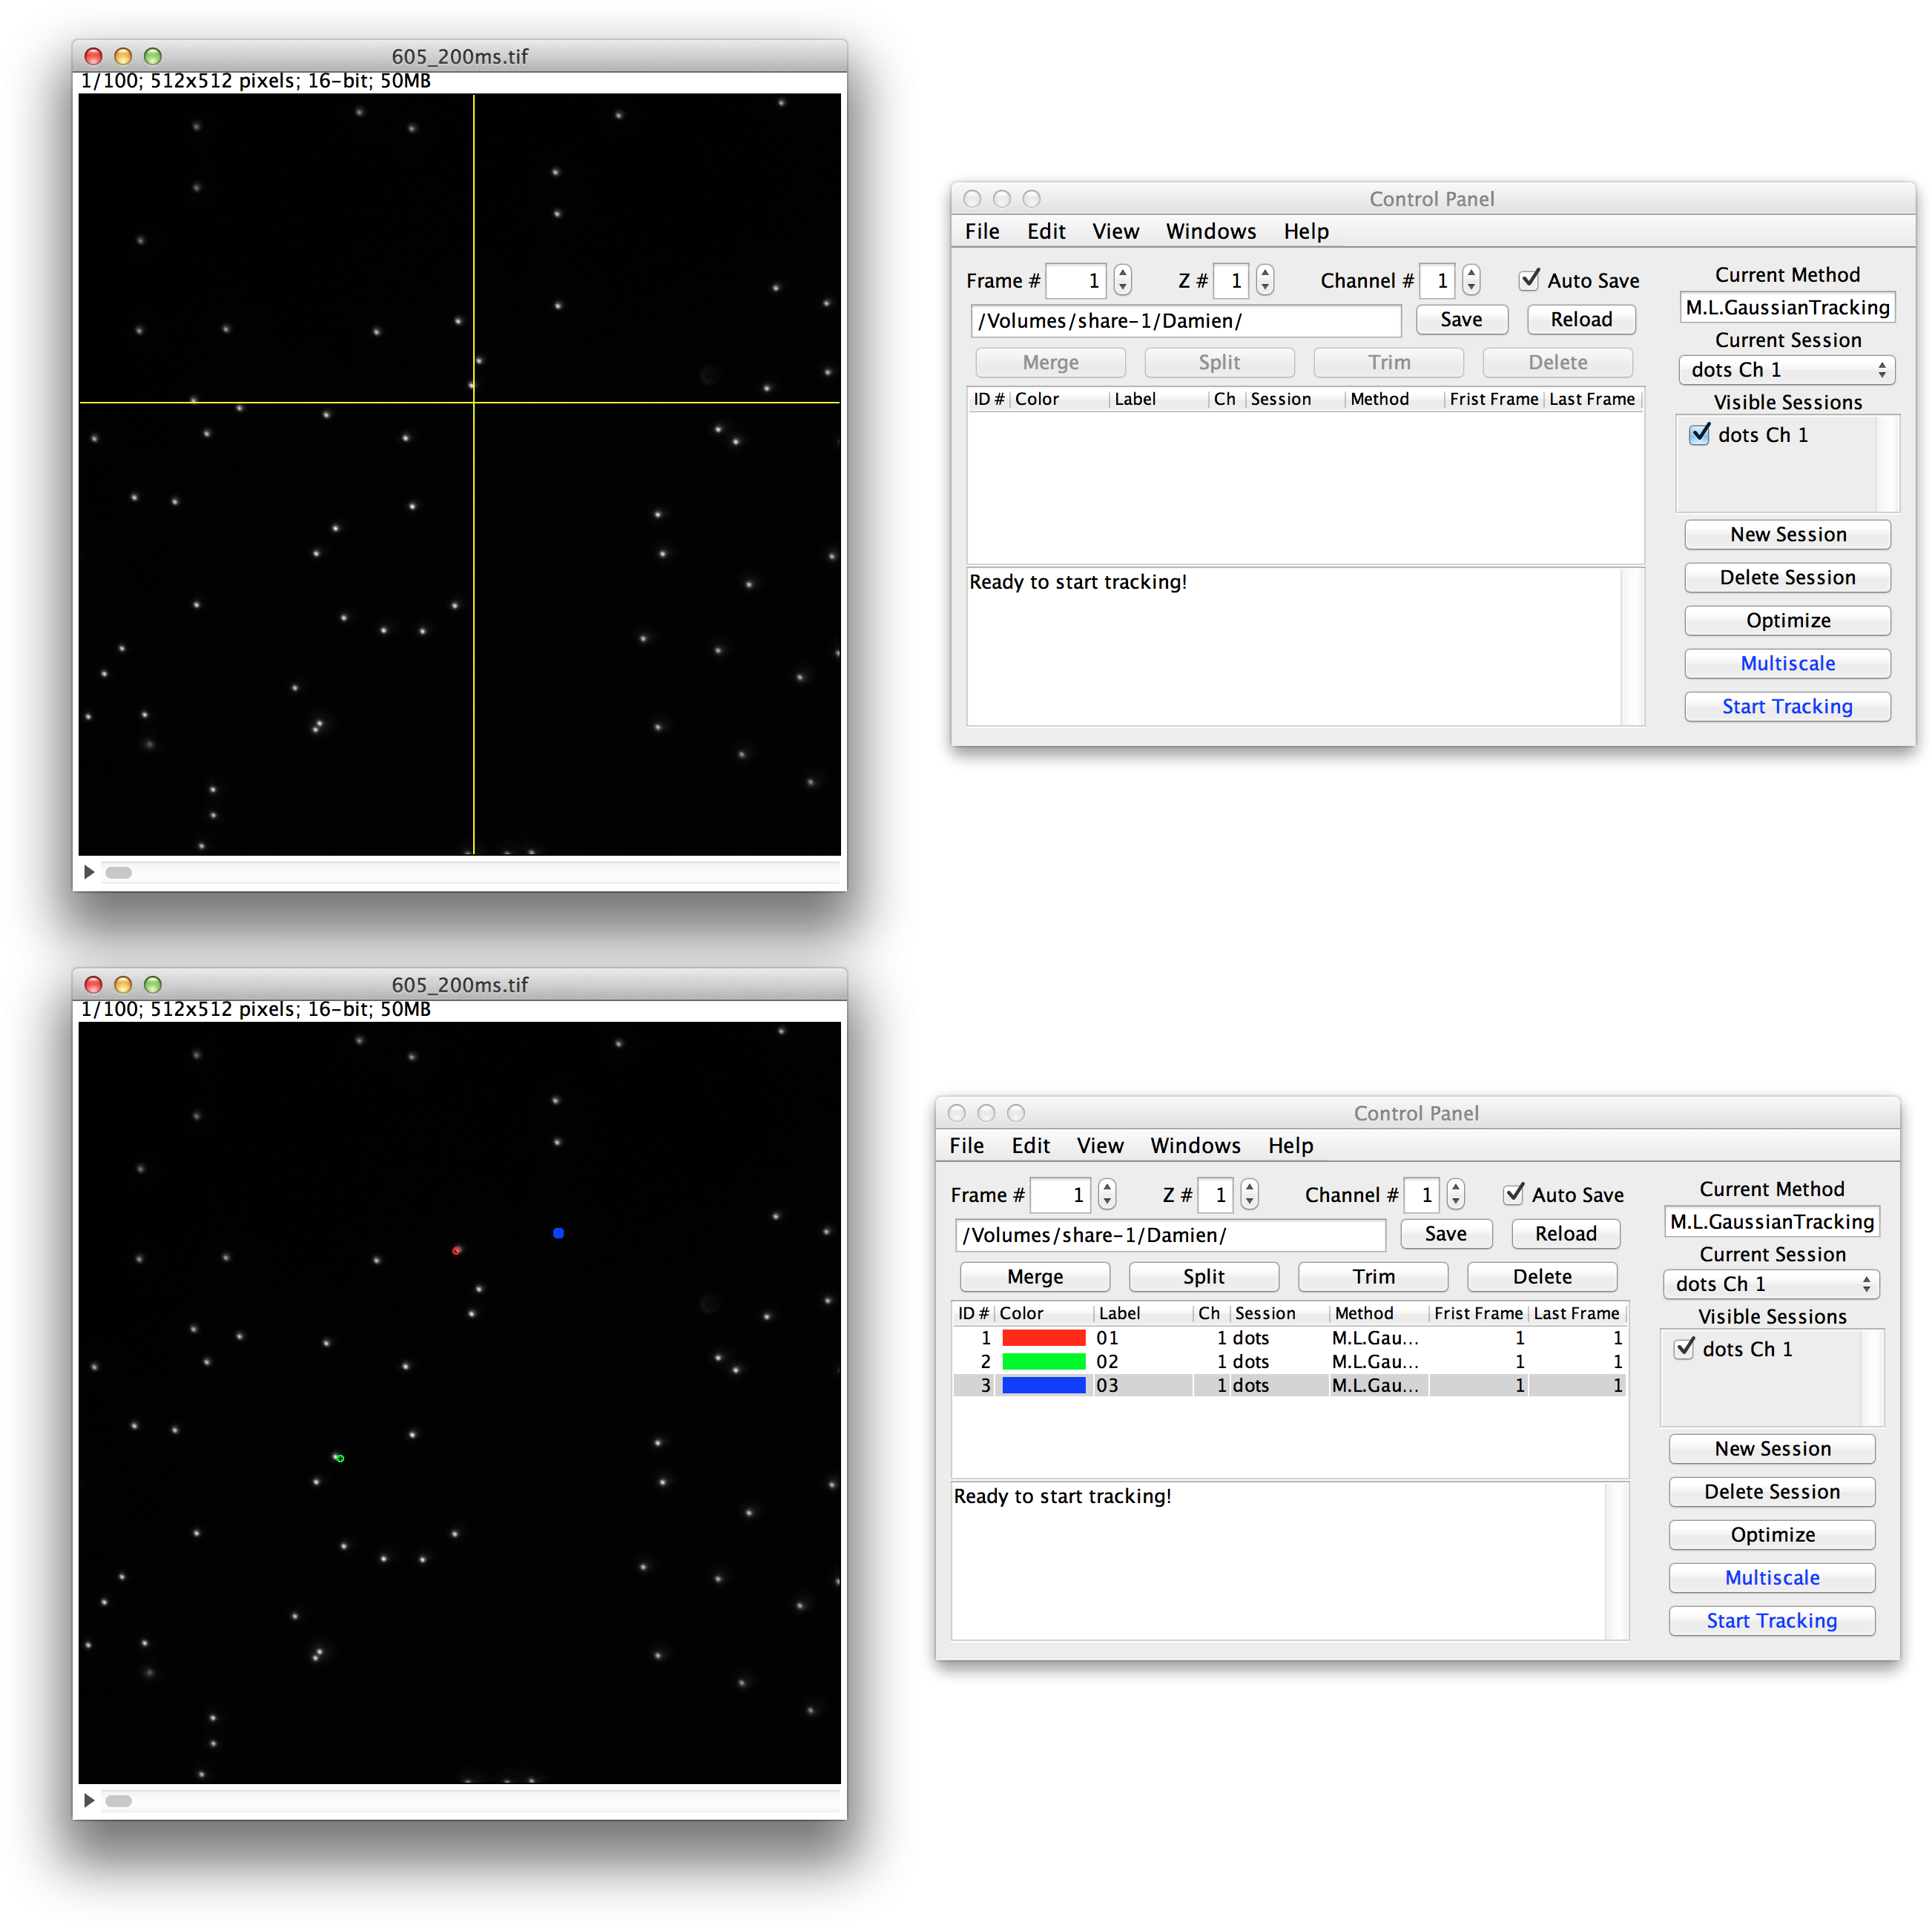
\includegraphics[width=5 in]{pickDots.png}
	\caption{Using the cross hairs on the image, double click to identify points to track. In the table you can rename each label, or change the color.  It is also possible to sort by each column }
	\label{pickDots}
\end{figure}


\section{3D time series}